\documentclass[a4paper,latin]{paper} 
\usepackage{babel}  
\usepackage[margin=2.5cm]{geometry}
\usepackage{graphicx}
\usepackage{lipsum}
\usepackage{xcolor}
\usepackage{booktabs}
\sectionfont{\large\sf\bfseries\color{black!70!blue}} 
\renewcommand\keywordname{Clavem verborum}
\title{Minimum exemplum laborandi}
\subtitle{Exemplum apparentia \texttt{paper} tabellae\\
\hfill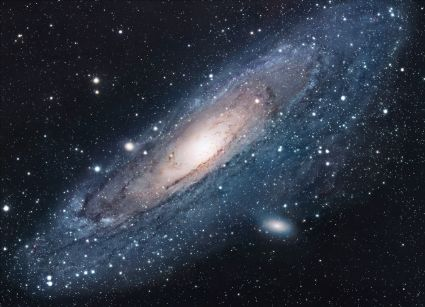
\includegraphics[height=2cm]{../02_Immagini/img_src/universe.jpg}
\vspace{-2cm}}
\author{Ph. D. Franciscus Studiosum Somniantis} 
\institution{Ignotum Universitas \\ 
Ad requiem centrum Scientiarum}


\begin{document} 
\twocolumn[\maketitle 
\hrule 
\smalltableofcontents
\begin{abstract} {\lipsum[12]} \end{abstract}
\begin{keywords}
MWE, \LaTeX, document class, \texttt{paper},
\texttt{article}, dummy text    
\end{keywords}
\hrule\bigskip
]


\section{Introduction} 
Some introduction. \lipsum[2]
\section{Materia et modos} 
More dummy text. \lipsum[4] 

\begin{table}[b]
\centering
\begin{tabular}{lcccccc}
\toprule
& I &  II & III & IV & V & VI \\
\midrule
Vandali     & 123 & 456 & 678 & 321 & 644 & 768  \\ 
Visigothorum & 021 & 229 & 678 & 123 & 456 & 678 \\     
\bottomrule
\end{tabular}
\caption{Visigothi cum Romanis foederati Hispaniam ingressi sunt et contra Vandalos. Mortem comitis utraque pugna.} 
\end{table}

\section{Consequitur} 
These are the results. \lipsum[1]
\section{Disputatio} 
\lipsum[4] 
\section{Conclusionibus}
\lipsum[5]
\end {document}